\chapter{Abstract Metric}\label{sec:absmetric}
There are numerous methods for evaluating the performance of players, as seen in section \ref{sec:ppm}. In machine learning, evaluation of agents plays an important role, to compare results. However, it is not an easy task to design suitable methodologies because agents can obtain misleading high scores due to overfitting test evaluations \cite{5967363}.

In this section, state-of-the-art evaluation metrics are discussed, and for the field of Arcade video games, new ones are introduced.


\section{State-of-the-art}
Even though agents share the same goal, maximizing scores, interpreting the results is difficult. This is due to various reasons; one of them is the variation of the scaling for the scores. For example, in one game, the player gets a reward of two for successfully collecting an item and in another game a reward of 10 \cite{MsPacMan87:online, FishingD32:online}. Additionally, different game mechanics make some games more complex than others \cite{2012arXiv1207.4708B}. In order to help compare agents across a broad set of fields, evaluation metrics, which include normalizing of scores and aggregation of scores, were introduced by \citeA{2012arXiv1207.4708B}.

\subsection{Normalizing Scores}
The concept behind the logic \cite{2012arXiv1207.4708B} is using to normalize scores is that it compares the scores of each algorithm, depending on a score range. The score range varies among the three types the authors had presented, which are normalization to a reference score, normalizing to a baseline set and inter-Algorithm normalization.
The equation for calculating a normalized score is defined by:
\begin{equation}
z_{g,i} := (s_{g,i} - r_{g,min}) / (r_{g,max} - r_{g,min})
\label{eq:norm_score}
\end{equation}
\myequations{Normalized score equation}

Since the scores for inter-algorithm are bounded, which is defined by\(z_{g, i}\in [0, 1]\), it is seen as an appealing solution to compare the relative performance of different methods. The score range for the inter-algorithm type is defined as $[min_{i \in \{1,\dots , n\}}  s_{g,i}, max_{i \in \{1,\dots , n\}} s_{g,i}]$.

However, it comes with a drawback; the best algorithm its objective performance cannot be seen, e.g. in the game \textit{Venture}, an algorithm achieved a score of 1.0. Still it was not even close to human performance. Therefore, the authors suggest, to use it as a complement to other metrics.

\subsection{Aggregating Scores}
To demonstrate how well agents perform across a collection of games, the normalized scores are aggregated. The authors present three ways, the average score, the median score and score distribution. 

The easiest way is to use the average of all normalized scores, but the issue with this approach is, that the measure can be affected by games with high scores. To avoid that, combining the value with the inter-algorithm is an option, as demonstrated in figure \ref{fig:5_agg_score}. 

The other approach is to use the median score, which is computed by initially sorting the normalized scores and select the number in the middle. If the number of scores is an even number, then the average of both middle numbers is used. 

By comparing the average, or mean, with the median values, the issue regarding an outlying score is visible in figure \ref{fig:5_agg_score}. The \textit{LSH} agents look like it performed very well, in contrast to the other agents, but this was due to a high score in one of the games.
\begin{figure}[H]%
\centering
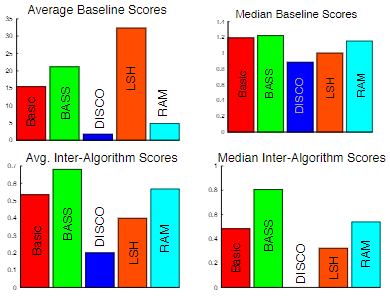
\includegraphics[width=8cm, height=6cm]{source/images/5_agg_score}%
\caption[Aggregation of normalized scores]{Aggregate normalized scores for the five reinforcement learning agents. Adapted from \protect\cite{2012arXiv1207.4708B}}%
\label{fig:5_agg_score}%
\end{figure}
The score distribution variant shows the percentage of games where an algorithm achieved a specific normalized score or higher. The benefit of this method is that it accurately shows the performance of an agent regardless of how other scores are distributed. Therefore, with this method, is it possible to compare algorithms, as seen in Figure \ref{fig:5_scr_dist}. The algorithm with the higher curve generally achieves higher scores.
\begin{figure}[H]%
\centering
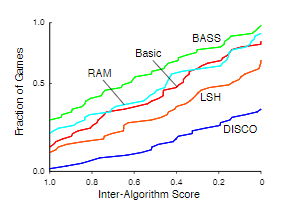
\includegraphics[width=8cm, height=6cm]{source/images/5_scr_dist}%
\caption{Score distribution. Source: Adapted from \protect\cite{2012arXiv1207.4708B}}
\label{fig:5_scr_dist}%
\end{figure}


\section{Arcade Games} \label{sec:arcgames}
In the toolkit OpenAI Gym (Gym), it is possible to develop and compare RL algorithms on different environments, such as the \textit{Atari} collection. Atari is a collection of environments consisting of video games for the Atari 2600 console \cite{1606.01540} by using the Atari Learning Environment from \citeA{2012arXiv1207.4708B}, which provides an interface for those games. The Atari environments are used for numerous algorithm research purposes, as seen in section \ref{sec:ai_agents}.

The evaluation metric for the agents in section \ref{sec:ai_agents} is the same in all Atari environments. All authors use the game score to determine their agents' performance. Varying attributes are, but not limited to, amount of games, game selection and the method used to display the score in a comparable manner, i.e., normalizing and aggregation of scores. \citeA{2018arXiv181207069P} collected the algorithms from section \ref{sec:ai_agents} and made a web tool to see how the different agents are performing. In the game Ms. Pacman, see section \ref{ssec:pacman}, the \nameref{ssec:rain} agent achieves a game score of 2180 in two runs (the third run is cut, due to length of the video, which is capped to 41 seconds)\footnote{\url{https://uber-research.github.io/atari-model-zoo/video.html?algo=rainbow&game=MsPacman&tag=final&run=1}}. Subsequently, the mean score for \nameref{ssec:es} is 3200\footnote{\url{https://uber-research.github.io/atari-model-zoo/video.html?algo=es&game=MsPacman&tag=final&run=1}}. It is clear that the \nameref{ssec:es} has a higher score than \nameref{ssec:rain}, but by watching the gameplays it is also clear that both agents are playing the game differently. The \nameref{ssec:rain} agent plays the game with the goal to finish the level, on the other hand, the \nameref{ssec:es} agent plays the game with the goal of eating as many ghosts as possible and ends up being stuck in a corner. Even though the \nameref{ssec:es} has a higher game score than \nameref{ssec:rain}, it does not necessarily mean that the \nameref{ssec:es} agent performed better than the \nameref{ssec:rain} agent, rather both agents have different objectives and ways to maximize their scores.

In other to address this issue, alternative metrics can be used, for example, the applicable ones from section \ref{sec:ppm}, which can be summarized as:
\begin{itemize}
	\item calculate the APM, or record the action-sequence
	\item usage of in-game stats
	\item splitting the game into sub-tasks
\end{itemize}
The remaining metrics are not necessarily applicable, due to differences in environments.

Those three metrics can be obtained to a certain degree. Calculating the APM is straight-forward, since it only requires to count how often an agents acts per minute. Whereas obtaining in-game stats is not that easy, because as previously mentioned, the Atari environment provides only the score as a reward, therefore it is essential to analyze the games and determine how scores are achieved. The sub-tasks for each game will vary, due to the reason that every game is different. However, some sub-tasks might be universal.

\citeA{Mnih2015} chose 49 Atari games for the evaluation of the \nameref{ssec:dqn}. The agent was able to play at human-level or above. Out of the 49 games, 10 were chosen for the analysis. The selection of the games is based on the performance of the DQN and subdivided into, below human-level, around human-level and above human-level. The following games were chosen for an in-depth analysis: Alien, Atlantis, Boxing, Centipede, Fishing Derby, Gopher, Ms. Pacman, Q-Bert, Sequest and Wizard of Wor.
Due to space limitations, only three games are explained
\subsection{Atlantis}
In Atlantis, the player has to defend a city from flying space ships. The city consists of six bases and three firing stations. The opposing ships are flying from top left (or right) to the other side of the screen, and each time they succeed, without getting destroyed by the player, they fly closer to the city, which is located at the bottom half of the screen. Eventually, the ships are using death rays to destroy the bases. The three firing stations are located in the most right, middle and most left part of the city. The middle one is firing straight upwards, while the left and the right one to the opposing direction. The ships can only destroy the bases when the firing station in the middle has been destroyed, t takes the end of a round for it to recover. Due to the variation of the ships, different scores are gained (100-3500). Also, the speed of the ships increases with time. The metrics for this game are:
\begin{itemize}
	\item action-sequence/APM
	\item aim
	\item amount of lives (bases)
	\item score value
\end{itemize}

\subsection{Fishing Derby}
In Fishing Derby, the goal is to achieve a score of 100 by fishing. Two players sit opposite themselves at the sides of the lake, with three fishes on each side. Due to their depth, the fishes give varying scores, which are 2, 4 and 6, respectively, according to their depth. Near the surface, a shark is waiting for the catch of the fishermen. The players have to avoid the shark to save as much time as possible. The metrics for this game are:
\begin{itemize} 
	\item action-sequence/APM
	\item completed level
	\item dodging
	\begin{itemize}
		\item shark
	\end{itemize}
	\item score value
	\item time steps
\end{itemize}

\subsection{Ms. Pacman} \label{ssec:pacman}
In Ms. Pacman, the player has to eat all \textit{pellets} in a maze, while avoiding the attacks of the four ghosts, which spawn one at a time. Pellets are dots on the screen, and there are in total 154. Four of them are \textit{power pellets}, which give the player the ability to eat ghosts for a specific time frame. By eating all pellets, the player is taken to the next level, with varying mazes in later stages of the game. The player gets ten points per pellet, 50 per power pellet and 200 points for a ghost. By eating ghosts successively, the amount of points is doubled each time. Starting with 200 for the first ghost, 400 for the second, 800 for the third and 1600 for the fourth. This can be done 4 times due to the number of power pellets. Twice per level, items referred to as fruits, are spawning and give increasing points throughout the game, starting with 100. The player has three lives and gets a bonus life at 10 000 points. The metrics for this game are:
\begin{itemize}
	\item action-sequence/APM
	\item amount of lives
	\item completed level
	\item dodging
	\item efficient pathing
	\begin{itemize}
		\item eating food
		\item eating pellets
		\item eating ghosts
	\end{itemize}
	\item score value
	\item time steps
\end{itemize}

Atari games have four common metrics. These are action-sequence/APM, amount of lives, amount of score and dodging. Section \ref{sec:exev} assesses whether these metrics are applicable for evaluation, or not.









